% concatenated from main.tex, preamble/packages.tex, preamble/macros.tex, preamble/theorems.tex, preamble/tikzstyles.tex, sections/sec00-abstract.tex, sections/sec01-intro.tex, sections/sec02-preliminaries.tex, sections/sec03-terminal-selection.tex, sections/sec04-fragile.tex, sections/sec05-conjectures.tex, sections/sec06-concluding.tex
\documentclass[a4paper,11pt]{article}

\usepackage{geometry}
\geometry{a4paper, left=2.4cm, right=2.4cm, top=2.6cm, bottom=2.6cm}
\linespread{1.05}
\usepackage{lmodern}

% packages.tex — package set and load order for the 3DC paper.
% NOTE: hyperref must load before cleveref, and cleveref must be LAST.

% --- math core ---
\usepackage{amsmath}
\usepackage{amssymb}
\usepackage{amsthm}
\usepackage{mathtools}
\usepackage{thmtools}
\allowdisplaybreaks           % long align blocks may break across pages

% --- graphics / figures ---
\usepackage{graphicx}
\usepackage{tikz}
\usetikzlibrary{arrows.meta,calc,positioning,decorations.pathreplacing,shapes}
\usepackage{caption}
\usepackage{subcaption}

% --- typography ---
\usepackage[T1]{fontenc}
\usepackage{microtype}
\usepackage[dvipsnames]{xcolor}
\usepackage[shortlabels]{enumitem}

% --- bibliography: self-contained thebibliography (no biber needed on arXiv) ---
% (References are typed directly in main.tex; see the thebibliography block.)

% --- cross-references: hyperref THEN cleveref, both last ---
\usepackage[colorlinks=true,linkcolor=BrickRed,citecolor=RoyalBlue,%
            urlcolor=RoyalBlue,linktocpage=true]{hyperref}
\usepackage[noabbrev,capitalize]{cleveref}
\crefname{equation}{}{}       % references to equations print as bare "(3.4)"
\Crefname{equation}{}{}

% macros.tex — notation macros for the 3DC paper.
% Also replaces the raw Unicode glyphs from the Markdown source (∎ ∪ ∖ △ ∅)
% with proper LaTeX under pdflatex.

% --- delimiters (Zhao-style) ---
\newcommand{\abs}[1]{\left\lvert#1\right\rvert}
\newcommand{\norm}[1]{\left\lVert#1\right\rVert}
\newcommand{\ang}[1]{\left\langle #1 \right\rangle}
\newcommand{\floor}[1]{\left\lfloor #1 \right\rfloor}
\newcommand{\ceil}[1]{\left\lceil #1 \right\rceil}

% --- blackboard sets ---
\newcommand{\RR}{\mathbb{R}}
\newcommand{\NN}{\mathbb{N}}
\newcommand{\ZZ}{\mathbb{Z}}

% --- graph-theoretic notation used throughout ---
\newcommand{\Vtwo}{V_2}                      % degree-two vertices (terminals)
\newcommand{\Vthree}{V_3}                     % degree-three vertices
\newcommand{\symdiff}{\mathbin{\triangle}}    % matching symmetric difference (source: \mathbin{\triangle})
\newcommand{\dcup}{\mathbin{\dot\cup}}         % disjoint union of edge sets (source: \dot\cup)
\newcommand{\empt}{\varnothing}                % empty set (source: ∅)
\DeclareMathOperator{\cyc}{\rho}               % cyclomatic number rho(L)

% Convenience: the target matching size q and the graph H-M complement notation
% are used verbatim from the source; no macro needed beyond the above.

% theorems.tex — theorem environments (shared counter, numbered within section)
% Defined with thmtools so cleveref names come for free. Load after amsthm/thmtools,
% before cleveref (order handled in main.tex via packages.tex).

\declaretheorem[name=Theorem,numberwithin=section]{theorem}
\declaretheorem[name=Lemma,sibling=theorem]{lemma}
\declaretheorem[name=Proposition,sibling=theorem]{proposition}
\declaretheorem[name=Corollary,sibling=theorem]{corollary}
\declaretheorem[name=Conjecture,sibling=theorem]{conjecture}

\declaretheorem[style=definition,name=Definition,sibling=theorem]{definition}
\declaretheorem[style=remark,name=Remark,sibling=theorem]{remark}
\declaretheorem[style=definition,name=Question,sibling=theorem]{question}

% Number equations within sections: (3.1), (3.4), ... matching the manuscript.
\numberwithin{equation}{section}

% tikzstyles.tex — vertex/edge styles for cubic/subcubic graph figures.
% Adapted from 04_references/reductions_source/3DC-reductions-single-file.tex
% so figures match the visual conventions of the subfield.

\tikzset{
  % a filled black vertex (generic / cubic vertex)
  cvertex/.style = {circle, draw=black, fill=black, inner sep=0pt, minimum size=1.6mm},
  % a terminal (degree-two) vertex: hollow, to stand out
  tvertex/.style = {circle, draw=black, fill=white, line width=0.7pt, inner sep=0pt, minimum size=2.2mm},
  % a new/auxiliary vertex introduced by a construction
  nvertex/.style = {circle, draw=black, fill=black!12, inner sep=0pt, minimum size=2.0mm},
  % ordinary graph edge
  gedge/.style   = {line width=0.8pt},
  % a matching edge: a single heavier solid line
  medge/.style   = {line width=1.7pt, line cap=round},
  % an edge that is deleted / removed (dashed)
  redge/.style   = {line width=0.8pt, dashed},
  % label font for figures
  glabel/.style  = {font=\footnotesize},
}
\tikzset{>=latex}

% A transformation arrow "==>" between before/after panels.
\newcommand{\transarrow}{\ensuremath{\longrightarrow}}


\title{Matching complements in subcubic graphs\\[2pt]
        and a proof of the 3-Decomposition Conjecture}

\author{Jicheng Ma\thanks{Corresponding author. School of Mathematics, Renmin
University of China, Beijing, 100872, China. Email:
\texttt{mjc191812@ruc.edu.cn}.}}

\date{}

\begin{document}

\maketitle

\begin{abstract}
We prove the $3$-Decomposition Conjecture: every finite connected cubic
loopless multigraph decomposes into a spanning tree, a $2$-regular subgraph, and
a matching. The proof rests on a new theorem on matching complements in
subcubic graphs. Let $H$ be a finite connected bridgeless simple graph of
maximum degree three, and let $S$ be its set of degree-two vertices, with
$\abs{S}=k\ge 2$. We show that $H$ has a matching of size equal to its
cyclomatic number, $\abs{E(H)}-\abs{V(H)}+1$, whose deletion leaves a single
tree containing all of $S$, together with cycles disjoint from $S$. The proof is
by induction on $k$, using an alternating-path exchange that stops at the first
entry into the growing tree component.

\end{abstract}

\noindent\textbf{Keywords.} 3-Decomposition Conjecture, cubic graph, graph
decomposition, spanning tree, matching, perfect matching.

\smallskip

\noindent\textbf{Mathematics Subject Classification (2020).} 05C70, 05C05.

\bigskip

% ---- section files (\input flows continuously; no forced page breaks) ----
\section{Introduction}\label{sec:intro}

A \emph{$3$-decomposition} of a graph $G$ is a partition of its edge set into a
spanning tree, a $2$-regular subgraph, and a matching. By Petersen's
theorem~\cite{Petersen1891}, every bridgeless cubic graph has a perfect matching,
and hence a $2$-factor. Malkevitch~\cite{Malkevitch1979} studied which cubic
graphs decompose into a spanning tree and a $2$-regular subgraph; for a cubic
graph this is equivalent to having a homeomorphically irreducible spanning tree,
that is, a spanning tree with no vertex of degree two. Allowing a matching as a
third part, Hoffmann-Ostenhof~\cite{HoffmannOstenhof2011} conjectured in 2011
that such a decomposition always exists.

\begin{conjecture}[3-Decomposition Conjecture~\cite{HoffmannOstenhof2011}]\label{conj:3dc}
  Every finite connected cubic loopless multigraph has an edge partition into a
  spanning tree, a $2$-regular subgraph, and a matching.
\end{conjecture}

Despite its elementary statement, the conjecture has been open for over a decade and has
become one of the central open problems on edge decompositions of cubic graphs.
It is equivalent, by Hoffmann-Ostenhof, Kaiser, and
Ozeki~\cite{HoffmannOstenhofKaiserOzeki2018}, to the \emph{$2$-Decomposition
Conjecture} (2DC): every connected loopless multigraph with all degrees two or
three, in which every cycle is separating, splits into a spanning tree and a
matching. Botler, Jim\'enez, Sambinelli, and
Wakabayashi~\cite{BotlerJimenezSambinelliWakabayashi2024} established strong
structural restrictions on a minimum counterexample to 2DC, proving in particular
that it must be simple and $2$-edge-connected.

Several results relax the matching to a union of vertex-disjoint paths of length
at most two. Hong, Liu, and Yu~\cite{HongLiuYu2020}, Li and
Cui~\cite{LiCui2014}, and Lyngsie and Merker~\cite{LyngsieMerker2019}
independently established such a decomposition for every connected cubic graph,
the last as a specialization of a tree, even graph, and star forest
decomposition. Fan and Zhou~\cite{FanZhou2025} then bounded the number of
length-two paths by $(n-4)/6$, and Fan, Guo, and Zhou~\cite{FanGuoZhou2026}
improved this to $(n-4)/8$; 3DC is exactly the assertion that this count can be
made zero. Zhang and Szeider~\cite{ZhangSzeider2025} verified the conjecture by
computer for all relevant graphs up to $28$ vertices.

The conjecture has also been confirmed for several families of graphs. The
planar case was settled by Hoffmann-Ostenhof, Kaiser, and
Ozeki~\cite{HoffmannOstenhofKaiserOzeki2018}, following the $3$-connected planar
case of Ozeki and Ye~\cite{OzekiYe2016}; it is known for traceable cubic
graphs~\cite{AbdolhosseiniAkbariHashemiMoradian2016, LiuLi2020}, for claw-free
or $4$-chordal subcubic graphs~\cite{AboomahigirAhanjidehAkbari2018}, for cubic
graphs having a $2$-factor consisting of three cycles~\cite{XieZhouZhou2020},
and for $3$-connected star-like graphs~\cite{BachtlerKrumke2022}. Bachtler and
Heinrich~\cite{BachtlerHeinrich2023} identified several reducible configurations
and proved the conjecture for $3$-connected cubic graphs of path-width at most
four. The surrounding matching-decycling problems were studied by Protti and
Souza~\cite{ProttiSouza2018}. The full conjecture has remained open.

In this paper we prove it.

\begin{theorem}\label{thm:3dc-resolved}
  The $3$-Decomposition Conjecture holds.
\end{theorem}

Rather than working with cubic graphs directly, we establish a new theorem on
matching complements in subcubic graphs, and deduce 3DC from it in two steps.
The matching argument uses the theorem of Petersen and Sch\"onberger that a
bridgeless cubic graph has a perfect matching through any prescribed edge: mere
existence of a perfect matching gives the one we need in the auxiliary cubic
graph, while the prescribed edge is used in the base case. The
passage to 2DC uses the elegant minimum-counterexample structure theorem of
Botler, Jim\'enez, Sambinelli, and
Wakabayashi~\cite{BotlerJimenezSambinelliWakabayashi2024}.

Call a graph in which every vertex has degree two or three a
\emph{$\{2,3\}$-graph}, and a degree-two vertex of such a graph a
\emph{terminal}; write $\Vtwo(H)$ for its set of terminals and $\Vthree(H)$ for
its set of degree-three vertices.

\begin{theorem}\label{thm:terminal-selection}
  Let $H$ be a finite connected bridgeless simple graph, every vertex of which
  has degree two or three. If $S=\Vtwo(H)$ with $\abs{S}=k\ge 2$, then $H$ has a
  matching $M$ of size
  \begin{equation}\label{eq:main-size}
    \abs{M}=q:=\frac{\abs{V(H)}-k+2}{2}
  \end{equation}
  such that $H-M$ is the disjoint union of one tree containing all vertices of
  $S$ and zero or more cycles.
\end{theorem}

The size in \cref{eq:main-size} equals the cyclomatic number
$\abs{E(H)}-\abs{V(H)}+1$, the only value for which the complement can be a
single tree together with cycles. The hypothesis $k\ge 2$ is necessary: when
$k=0$ or $k=1$ one has $q>\abs{V(H)}/2$, so no matching of the prescribed size
exists. No upper bound on $k$ is imposed.

A cycle $C$ in a connected graph $G$ is \emph{separating} if $G-E(C)$ is
disconnected, and $G$ is \emph{fragile} when every one of its cycles is
separating. \Cref{thm:terminal-selection} yields the following consequence,
again with no bound on the number of degree-two vertices, proved in
\cref{sec:fragile}.

\begin{theorem}\label{thm:simple-fragile}
  Every finite connected simple fragile subcubic graph admits an edge partition
  into a spanning tree and a matching.
\end{theorem}

Two further steps close the gap to 3DC. Every counterexample to 2DC is, by
definition, a connected fragile $\{2,3\}$-graph; by Botler, Jim\'enez, Sambinelli,
and Wakabayashi~\cite{BotlerJimenezSambinelliWakabayashi2024}, one minimizing
$\abs{V(G)}+\abs{E(G)}$ is moreover simple, so \cref{thm:simple-fragile} applies
and rules it out. This proves 2DC in its standard loopless-multigraph form
(\cref{sec:2dc-interface}); a direct maximal-cycle and $2$-core construction then
carries 2DC to 3DC (\cref{sec:2dc-to-3dc}). In these two steps we
work with loopless multigraphs, so that parallel edges are allowed and a
parallel pair counts as a cycle of length two.

\subsection*{Overview of the proof}

We prove \cref{thm:terminal-selection} by strong induction on $k$.

\emph{Counting.}  A handshaking argument (\cref{sec:counting}) shows that the
target size $q=(n-k+2)/2$ is the unique value for which the complement can be a
tree together with cycles.  For a matching of size $q$, the \emph{component
identity} $z(L)-t(L)=2\cyc(L)-2$ (where $z$, $t$, $\cyc$ count exposures,
terminals, and cyclomatic number in a component $L$) reduces the problem to placing all
terminals in a single component.

\emph{Normalizations.}  In a minimum counterexample with $k$ terminals, two
local reductions (\cref{sec:normalizations}) enforce that no two terminals are
adjacent and every terminal can be suppressed without creating a loop or a
parallel edge.

\emph{Comparison matching.}  To choose which terminal to suppress, we attach all
$k$ terminals to an arbitrary full cubic tree $\mathcal T$ with $k-2$ internal
vertices, forming a cubic graph $\widehat H$ (\cref{sec:cubic-tree}).  A
perfect matching $P$ of $\widehat H$ restricts to a matching $N=P\cap E(H)$ of
size $q+r$ ($r\ge 0$) that covers every cubic vertex and at least two terminals.

\emph{First-entry transfer.}  Suppressing a terminal $s$ covered by $N$, applying
the induction hypothesis to the smaller graph $J$, and restoring $s$ yields four
cases (\cref{sec:first-entry}): two finish directly, and two leave a single
vertex $x$ outside the growing tree component $Q$.  In these two cases, $x$ is
$N$-covered and every $N$-exposure is already in $Q$, so a symmetric-difference
path from $x$ must re-enter $Q$ at some first vertex $d$.  Flipping along the
prefix $x\cdots d$ (which contains equally many edges of each matching)
moves the exposure outside $Q$ into $Q$ without removing any complement edge
inside $Q$.
The parity identity then forces $s$ into $Q'$, closing the induction regardless
of the value of $r$.

\subsection*{Organization}

\Cref{sec:prelim} fixes conventions and recalls the external results we use.
\Cref{sec:terminal-selection} proves \cref{thm:terminal-selection}.
\Cref{sec:fragile} deduces \cref{thm:simple-fragile}, and
\cref{sec:conjectures} passes from it to 2DC and then to 3DC.
\Cref{sec:scope} collects concluding remarks and open problems.

\section{Preliminaries}\label{sec:prelim}

All graphs in this paper are finite. For a matching $M$, a vertex is
\emph{covered} if it is incident with an edge of $M$, and \emph{exposed}
otherwise. Deleting a set of edges never deletes vertices. A $2$-regular
subgraph need not be spanning and may be empty, unless nonemptiness is
explicitly required. For a connected graph $L$ we write
$\cyc(L)=\abs{E(L)}-\abs{V(L)}+1$ for its cyclomatic number. We write $A\dcup B$ for the
union of two edge-disjoint edge sets, used to emphasise that the union is
disjoint.

\begin{theorem}[Sch\"onberger; Boyd--Iwata--Takazawa]\label{thm:specified-edge}
  If $K$ is a finite bridgeless cubic loopless multigraph and $e\in E(K)$,
  then $K$ has a perfect matching containing $e$.
\end{theorem}

This strengthening of Petersen's theorem is due to
Sch\"onberger~\cite{Schonberger1935}; we use the statement as given by Boyd, Iwata,
and Takazawa~\cite[Theorem~2.1]{BoydIwataTakazawa2013}, which allows parallel
edges. In particular, every finite bridgeless cubic loopless multigraph has a
perfect matching.

\begin{theorem}[Borse--Waphare~\cite{BorseWaphare2013}]\label{thm:protected-cycle}
  Let $G$ be a connected simple graph and let $Q$ be a connected subgraph.
  Suppose that $G$ contains a cycle edge-disjoint from $Q$, and that every
  $v\in V(G)\setminus V(Q)$ satisfies $d_G(v)\ge 3$. Then $G$ contains a cycle
  $C$ edge-disjoint from $Q$ such that $G-E(C)$ is connected.
\end{theorem}

Borse and Waphare~\cite{BorseWaphare2013} state this, attributing it to their
earlier work~\cite{BorseWaphare2009}; we include a short self-contained proof.

\begin{proof}
  Let $\mathcal H$ be the family of connected subgraphs $H$ of $G$ such that
  $Q\subseteq H$ and the spanning edge-complement
  \[
    F_H=\bigl(V(G),\,E(G)\setminus E(H)\bigr)
  \]
  contains a cycle. The hypothesised witness cycle shows that
  $Q\in\mathcal H$. Since $G$ is finite, choose $H\in\mathcal H$ with
  $\abs{E(H)}$ maximum, and write $F=F_H$.

  Every component of $F$ meets $V(H)$. Otherwise a shortest $G$-path from such
  a component to $V(H)$ would, up to its first vertex in $V(H)$, use only edges
  outside $E(H)$; it would therefore be an $F$-path joining the component to
  $V(H)$, a contradiction.

  Choose a component of $F$ that contains a cycle. It meets $V(H)$ and is
  nontrivial, so it has an edge $e\in E(F)$ incident with a vertex of $H$. The
  subgraph $H+e$, including the other endpoint of $e$ if necessary, is
  connected and contains $Q$. Maximality of $H$ forces $F-e$ to be acyclic,
  for otherwise $H+e$ would be a member of $\mathcal H$ with more edges. Thus
  $F-e$ is a forest. Since $F$ contains a cycle, adding the single edge $e$ to
  that forest creates exactly one cycle, which we denote by $C$. In
  particular, $C$ is edge-disjoint from $H$, and hence from $Q$.

  It remains to prove that $G-E(C)$ is connected. Suppose a component $D$ of
  the forest $F-E(C)$ does not meet $V(H)$. The component of $F$ containing $D$
  does meet $V(H)$, so $D$ contains a vertex of $C$; otherwise $D$ would
  already be an $F$-component. It contains at most one such vertex: if there
  were two or more, choose two at minimum distance in $D$. Their $D$-path has
  no internal vertex on $C$, and together with either arc of $C$ it would give
  a second cycle in $F$. Consequently
  \[
    V(D)\cap V(C)=\{x\}
  \]
  for some vertex $x$.

  Every vertex of $D$ lies outside $V(H)$, hence outside $V(Q)$, and every edge
  of $G$ incident with such a vertex belongs to $F$. No cycle edge is incident
  with a vertex of $D-\{x\}$, while exactly the two edges of the simple cycle
  $C$ incident with $x$ were deleted. Therefore
  \[
    d_D(v)=d_G(v)\ge 3\quad(v\in V(D)\setminus\{x\}),
    \qquad
    d_D(x)=d_G(x)-2\ge 1.
  \]
  Writing $m=\abs{V(D)}$ and using that $D$ is a finite tree gives
  \[
    2(m-1)=\sum_{v\in V(D)}d_D(v)\ge 1+3(m-1)=3m-2,
  \]
  which forces $m\le 0$, a contradiction. Hence every component of $F-E(C)$
  meets the connected subgraph $H$. Their union with $H$ is precisely
  $G-E(C)$, and is connected. This proves the theorem.
\end{proof}

\begin{theorem}[Botler--Jim\'enez--Sambinelli--Wakabayashi~\cite{BotlerJimenezSambinelliWakabayashi2024}]\label{thm:min-counterexample}
  Among connected fragile loopless multigraphs that are $\{2,3\}$-graphs, a
  counterexample to the $2$-Decomposition Conjecture minimizing
  $\abs{V(G)}+\abs{E(G)}$, if one exists, is simple and $2$-edge-connected.
\end{theorem}

This is item~(1) of \cite[Theorem~1.5]{BotlerJimenezSambinelliWakabayashi2024},
whose setting, like ours in \cref{sec:2dc-interface,sec:2dc-to-3dc}, permits
parallel edges, forbids loops, and treats a parallel pair as a cycle of length
two.

The loopless-multigraph forms of 2DC and 3DC are equivalent, by
Hoffmann-Ostenhof--Kaiser--Ozeki
\cite[Proposition~14]{HoffmannOstenhofKaiserOzeki2018}. We prove the direction
we need, that 2DC implies 3DC, in \cref{sec:2dc-to-3dc}.

\section{Terminal selection}\label{sec:terminal-selection}

The proof of \cref{thm:terminal-selection} is by strong induction on the number
$k$ of terminals.

\subsection{Counting inside a matching complement}\label{sec:counting}

Let $H$ be a $\{2,3\}$-graph, put $n=\abs{V(H)}$, and let $k=\abs{\Vtwo(H)}$.
The handshaking identity gives
\[
  2\abs{E(H)}=2k+3(n-k)=3n-k.
\]
Consequently $n-k=\abs{\Vthree(H)}$ is even and
\[
  \abs{E(H)}-\abs{V(H)}+1=\frac{n-k+2}{2}=\frac{\abs{\Vthree(H)}}{2}+1.
\]
Thus the target size
\[
  q:=\frac{\abs{V(H)}-k+2}{2}
\]
is an integer and $q\ge 1$. A matching of size $q$
covers $2q=n-k+2$ vertices, and therefore exposes exactly
\begin{equation}\label{eq:exposed}
  n-2q=k-2
\end{equation}
vertices.

Let $M$ be any
matching of $H$, and let $L$ be a component of $H-M$. Define
\[
  t(L)=\abs{V(L)\cap \Vtwo(H)},
  \qquad
  z(L)=\abs{\{v\in V(L):v\text{ is exposed by }M\}},
\]
and recall the cyclomatic number $\cyc(L)=\abs{E(L)}-\abs{V(L)}+1$.

\begin{lemma}\label{lem:component-identity}
  For every component $L$ of $H-M$,
  \begin{equation}\label{eq:component-identity}
    z(L)-t(L)=2\cyc(L)-2.
  \end{equation}
\end{lemma}

\begin{proof}
  A covered terminal has degree one in $H-M$, an exposed terminal has degree
  two, a covered cubic vertex has degree two, and an exposed cubic vertex has
  degree three. Hence the sum of $d_L(v)-2$ over $V(L)$ equals the number of
  exposed cubic vertices minus the number of covered terminals, which is
  exactly $z(L)-t(L)$. On the other hand,
  \[
    \sum_{v\in V(L)}\bigl(d_L(v)-2\bigr)=2\abs{E(L)}-2\abs{V(L)}=2\cyc(L)-2.
  \]
  Comparing the two expressions proves \cref{eq:component-identity}.
\end{proof}

\begin{lemma}\label{lem:terminal-criterion}
  Let $k\ge 2$ and let $M$ be a matching of size $q$. Then the following are
  equivalent.
  \begin{enumerate}[(i)]
    \item All $k$ terminals lie in one component of $H-M$.
    \item The graph $H-M$ consists of one tree containing all terminals and
      zero or more cycles containing no terminal.
  \end{enumerate}
  Moreover, all $k-2$ exposed vertices then lie in the distinguished tree.
\end{lemma}

\begin{proof}
  Condition~(ii) plainly implies~(i). Conversely, let $L$ be the component
  containing all $k$ terminals. By \cref{eq:exposed}, $z(L)\le k-2$. Identity
  \cref{eq:component-identity} together with $\cyc(L)\ge 0$ gives
  $z(L)\ge k-2$. Thus $z(L)=k-2$ and $\cyc(L)=0$, so $L$ is a tree and contains
  every exposed vertex. Any other component $R$ has $t(R)=z(R)=0$, whence
  $\cyc(R)=1$. Every vertex of $R$ is a covered cubic vertex, and hence has
  degree two in $H-M$. Therefore $R$ is a cycle.
\end{proof}

\subsection{Preparing a minimum counterexample}\label{sec:normalizations}

Fix $k\ge 3$, assume \cref{thm:terminal-selection} for
$k-1$, and, for contradiction, let $H$ be a counterexample with $k$ terminals
and the fewest possible vertices. The induction hypothesis then applies at
every order with $k-1$ terminals, while minimality of order applies to any
smaller graph with the same number $k$ of terminals.

\medskip\noindent\textbf{Reduction 1: no two terminals are adjacent.}

Suppose two terminals $u,v$ are adjacent. Let $x$ and $y$ be their respective
other neighbours. If $x=y$ is cubic, its third edge is the only edge from the
triangle $uvx$ to the rest of the graph, hence a bridge. If $x=y$ has degree
two, connectedness makes $H=C_3$, for which any one-edge matching leaves a
spanning path. Neither possibility occurs in the chosen counterexample, so
$x\ne y$.

Contract $uv$ to a new vertex $w$, retaining the edges $wx,wy$
(\cref{fig:reduction-adjacent}). The resulting graph $H_1$ is connected,
simple, bridgeless, and has $k-1$ terminals. It is simple because $x\ne y$;
bridgelessness follows by contracting $uv$ inside a cycle through each surviving
edge. Its target size is unchanged,
\[
  \frac{(\abs{V(H)}-1)-(k-1)+2}{2}=q .
\]
Apply the induction hypothesis to $H_1$, and let $Q$ be its tree component
containing all terminals. Since $w$ is a terminal, at most one of $wx,wy$ lies
in the selected matching, and the following three lifts are exhaustive.
\begin{itemize}
  \item If neither edge is matched, replace the tree path $xwy$ by $xuvy$.
  \item If $wx$ is matched, replace $wx$ in the matching by $xu$, and replace
    the tree leaf $yw$ by the path $yvu$.
  \item If $wy$ is matched, use the symmetric lift.
\end{itemize}
Each lift preserves the matching cardinality, expands only a path or a leaf of
$Q$, and leaves every residual cycle unchanged. It yields the desired
decomposition of $H$, a contradiction. Thus the terminal set of $H$ is
independent.

\begin{figure}[ht]
  \centering
  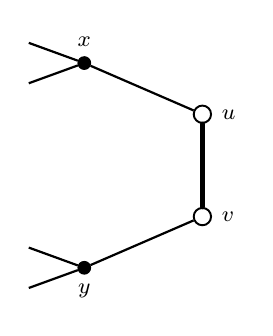
\begin{tikzpicture}[baseline]
    % before: two adjacent terminals u,v with other neighbours x,y
    \node[tvertex,label={[glabel]right:$u$}] (u) at (0,0.65) {};
    \node[tvertex,label={[glabel]right:$v$}] (v) at (0,-0.65) {};
    \node[cvertex,label={[glabel]above:$x$}] (x) at (-1.5,1.3) {};
    \node[cvertex,label={[glabel]below:$y$}] (y) at (-1.5,-1.3) {};
    \draw[medge] (u) -- (v);
    \draw[gedge] (u) -- (x);
    \draw[gedge] (v) -- (y);
    \draw[gedge] (x) -- ++(160:0.75); \draw[gedge] (x) -- ++(200:0.75);
    \draw[gedge] (y) -- ++(160:0.75); \draw[gedge] (y) -- ++(200:0.75);
  \end{tikzpicture}
  \qquad\transarrow\qquad
  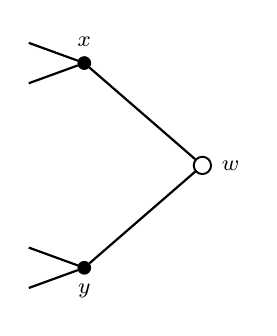
\begin{tikzpicture}[baseline]
    % after: contracted vertex w adjacent to x,y
    \node[tvertex,label={[glabel]right:$w$}] (w) at (0,0) {};
    \node[cvertex,label={[glabel]above:$x$}] (x) at (-1.5,1.3) {};
    \node[cvertex,label={[glabel]below:$y$}] (y) at (-1.5,-1.3) {};
    \draw[gedge] (w) -- (x);
    \draw[gedge] (w) -- (y);
    \draw[gedge] (x) -- ++(160:0.75); \draw[gedge] (x) -- ++(200:0.75);
    \draw[gedge] (y) -- ++(160:0.75); \draw[gedge] (y) -- ++(200:0.75);
  \end{tikzpicture}
  \caption{Removing an adjacency between terminals: the edge $uv$ (heavy) is
  contracted to a single terminal $w$. Hollow nodes are terminals; solid nodes
  are cubic.}
  \label{fig:reduction-adjacent}
\end{figure}

\medskip\noindent\textbf{Reduction 2: every terminal is suppressible.}

Let a terminal $s$ have neighbours $a,b$, and suppose $ab\in E(H)$. Terminal
independence makes $a,b$ cubic. Let $x$ and $y$ be their third neighbours. If
$x=y$ is cubic, its third edge is the sole edge leaving the four-vertex subgraph
on $s,a,b,x$, hence a bridge. If $x=y$ has degree two, connectedness makes this
four-vertex subgraph all of $H$, with exactly two terminals, contrary to
$k\ge 3$. Therefore $x\ne y$.

Replace the triangle $sab$ by a new degree-two vertex $w$ adjacent to $x,y$
(\cref{fig:reduction-triangle}). The graph $H_2$ is connected, bridgeless and
simple: cycles through the replaced triangle contract to cycles through $w$, and
all other cycles survive. It has $k$ terminals, two fewer vertices, and target
size $q-1$. Minimality of order therefore supplies a matching of size $q-1$
whose complement has an all-terminal tree $Q$ and cycles. Again there are three
states at $w$.
\begin{itemize}
  \item If neither $wx$ nor $wy$ is matched, add $ab$ to the matching and
    replace the tree path $xwy$ by $xasby$.
  \item If $wx$ is matched, replace it by the two disjoint matching edges
    $ax,sb$, and replace the tree leaf $yw$ by $ybas$.
  \item If $wy$ is matched, use the symmetric construction.
\end{itemize}
Each lift adds exactly one matching edge, as required when two vertices are
restored, and expands only a path or leaf of $Q$. This again contradicts the
choice of $H$. Hence every terminal of $H$ has two distinct cubic neighbours
that are nonadjacent; in particular, every terminal can be suppressed without
creating a loop or a parallel edge.

\begin{figure}[ht]
  \centering
  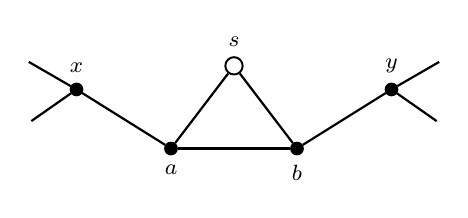
\begin{tikzpicture}[baseline]
    % before: terminal s with cubic a,b joined by edge ab, third neighbours x,y
    \node[tvertex,label={[glabel]above:$s$}] (s) at (0,1.05) {};
    \node[cvertex,label={[glabel]below:$a$}] (a) at (-0.8,0) {};
    \node[cvertex,label={[glabel]below:$b$}] (b) at (0.8,0) {};
    \node[cvertex,label={[glabel]above:$x$}] (x) at (-2.0,0.75) {};
    \node[cvertex,label={[glabel]above:$y$}] (y) at (2.0,0.75) {};
    \draw[gedge] (s) -- (a);
    \draw[gedge] (s) -- (b);
    \draw[gedge] (a) -- (b);
    \draw[gedge] (a) -- (x);
    \draw[gedge] (b) -- (y);
    \draw[gedge] (x) -- ++(150:0.7); \draw[gedge] (x) -- ++(215:0.7);
    \draw[gedge] (y) -- ++(30:0.7);  \draw[gedge] (y) -- ++(325:0.7);
  \end{tikzpicture}
  \qquad\transarrow\qquad
  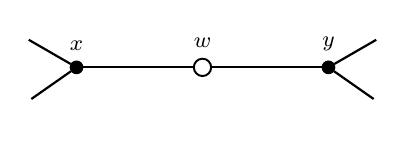
\begin{tikzpicture}[baseline]
    % after: degree-two w adjacent to x,y
    \node[tvertex,label={[glabel]above:$w$}] (w) at (0,0.75) {};
    \node[cvertex,label={[glabel]above:$x$}] (x) at (-1.6,0.75) {};
    \node[cvertex,label={[glabel]above:$y$}] (y) at (1.6,0.75) {};
    \draw[gedge] (w) -- (x);
    \draw[gedge] (w) -- (y);
    \draw[gedge] (x) -- ++(150:0.7); \draw[gedge] (x) -- ++(215:0.7);
    \draw[gedge] (y) -- ++(30:0.7);  \draw[gedge] (y) -- ++(325:0.7);
  \end{tikzpicture}
  \caption{Making a terminal suppressible: the triangle $sab$ is replaced by a
  single terminal $w$ joined to the two outer neighbours $x,y$.}
  \label{fig:reduction-triangle}
\end{figure}

\subsection{A comparison matching from a cubic tree}\label{sec:cubic-tree}

Throughout this section $H$ is a normalized graph as prepared in
\cref{sec:normalizations}: its terminal set is independent, and every terminal
has two distinct nonadjacent cubic neighbours.

For every $k\ge 3$ there is a tree $\mathcal T$ with exactly $k$ leaves and with
degree three at every nonleaf vertex. For example, begin with a claw at $k=3$,
and to add one leaf subdivide a leaf edge and attach a new leaf at the
subdivision vertex. The handshaking identity for a tree shows that $\mathcal T$
has exactly $k-2$ internal vertices.

Label the leaves of $\mathcal T$ by the $k$ terminals of $H$ and identify each
leaf with its corresponding terminal; all internal vertices of $\mathcal T$ are
new. Write
\[
  \widehat H=H\cup\mathcal T .
\]
This graph is simple and cubic. It is also bridgeless. Every old edge lies on an
old cycle. If $g\in E(\mathcal T)$, then each component of $\mathcal T-g$
contains a terminal leaf: otherwise one component would be a finite tree with no
vertex of degree one. Choose terminal leaves $u,v$ on opposite sides of $g$. A
simple $u$--$v$ path in $H$ and the unique $u$--$v$ path in $\mathcal T$ meet
only at $u,v$, since the internal tree vertices are new and no terminal leaf is
an internal vertex of a tree path. Their union is a cycle through $g$. Thus
every edge of $\widehat H$ lies on a cycle.

Choose a perfect matching $P$ of $\widehat H$ by \cref{thm:specified-edge}. Let
$I$ be the set of the $k-2$ new internal vertices, and set
\[
  r=\abs{P\cap E(\mathcal T[I])},
  \qquad
  p=\abs{\{e\in P:e\text{ joins a terminal to }I\}} .
\]
Counting how $P$ covers the internal vertices gives
\[
  2r+p=k-2 .
\]

Restrict $P$ to the original graph, $N=P\cap E(H)$. Every old cubic vertex is
covered by $N$. A terminal is exposed by $N$ exactly when its tree spoke belongs
to $P$, so precisely $p$ terminals are exposed. Since
$\abs{V(\widehat H)}=n+k-2$,
\begin{equation}\label{eq:N-size}
  \begin{aligned}
    \abs{N}
      &=\frac{n+k-2}{2}-(r+p)\\
      &=\frac{n-k+2}{2}+r=q+r .
  \end{aligned}
\end{equation}
The number of terminals covered by $N$ is
\begin{equation}\label{eq:covered-terminals}
  k-p=2+2r\ge 2 .
\end{equation}
No identity of an exposed terminal has been prescribed, and $r$ need not equal
one. The argument in \cref{sec:first-entry} selects a covered terminal only
after $N$ is known.

\subsection{First entry and the induction}\label{sec:first-entry}

\begin{lemma}\label{lem:first-entry}
  Let $M,N$ be matchings of a finite loopless graph $G$, let $Q$ be a component
  of $G-M$, and let $x\notin V(Q)$. Assume that
  \begin{itemize}
    \item $x$ is exposed by $M$ and covered by $N$;
    \item every other vertex exposed by $M$ belongs to $Q$; and
    \item every vertex exposed by $N$ belongs to $Q$.
  \end{itemize}
  Then there is a matching $M'$ with $\abs{M'}=\abs{M}$ such that the component
  of $G-M'$ containing $Q$ contains every vertex exposed by $M'$.
\end{lemma}

\begin{proof}
  In $M\symdiff N$, the vertex $x$ has degree one, and its incident edge belongs
  to $N\setminus M$. Its component is therefore a simple alternating path. The
  other endpoint is exposed by exactly one of $M,N$, and hence belongs to $Q$ by
  the hypotheses.

  Traverse the path from $x$, and stop at its first vertex $d\in V(Q)$. The edge
  that enters $Q$ must belong to $M\setminus N$: if it lay outside $M$, it would
  be an edge of $G-M$ joining its preceding outside vertex to the component $Q$,
  contrary to the choice of $Q$. Thus the prefix from $x$ to $d$ begins with an
  $N\setminus M$ edge and ends with an $M\setminus N$ edge, and it contains
  equally many edges of the two matchings.

  Flip membership along this prefix. The result $M'$ is a matching of the same
  size as $M$; it covers $x$ and exposes $d$. The prefix meets $Q$ for the first
  time at $d$, so no complement edge internal to $Q$ is removed, and the final
  $M$-edge becomes a complement edge entering $Q$. Every old $M$-exposure except
  $x$ remains in $Q$, and the only new exposure is $d\in Q$. Hence all
  $M'$-exposures lie in the component containing $Q$.
\end{proof}

\medskip\noindent\textbf{The base case $k=2$.}
Let $S=\{s,t\}$. Add a new edge $e=st$, allowing it to be parallel to an
existing $st$-edge. The resulting graph $K$ is a cubic loopless multigraph, and
it is bridgeless: old edges remain on old cycles, and an $s$--$t$ path in $H$,
together with $e$, is a cycle (a two-cycle when the path is an existing
$st$-edge).

Choose an old edge $f$ incident with $s$. By \cref{thm:specified-edge}, $K$ has
a perfect matching $M$ containing $f$. The matching cannot also contain the adjacent new edge $e$, so
$M\subseteq E(H)$ and $M$ is a perfect matching of $H$. Its cardinality is
$n/2=q$. In $H-M$, the vertices $s,t$ have degree one and every other vertex has
degree two. Therefore $H-M$ is one $s$--$t$ path together with zero or more
cycles. This proves the theorem for $k=2$, including the case in which the
completion has parallel edges.

\medskip\noindent\textbf{The inductive step $k\ge 3$.}
Assume \cref{thm:terminal-selection} for all smaller terminal counts, and suppose a $k$-terminal
counterexample exists. Choose one of minimum order. The reductions of
\cref{sec:normalizations} apply: its terminals are independent and every
terminal has two nonadjacent cubic neighbours.

Build the cubic-tree comparison matching $N$ of \cref{sec:cubic-tree}. By
\cref{eq:covered-terminals}, at least two terminals are covered by $N$. Choose
one such terminal $s$, and denote its neighbours in $H$ by $a,b$. Suppress $s$:
delete $s$ and add the edge $e=ab$. Call the resulting graph $J$. The
normalization ensures that $J$ is simple and remains a $\{2,3\}$-graph with
$k-1$ terminals. It is connected and bridgeless: since either incident edge at
$s$ lies on a cycle, $H-s$ contains an $a$--$b$ path; every cycle avoiding $s$
survives; a cycle using the segment $asb$ becomes a cycle using $ab$; and the
new edge $ab$ itself lies on such a cycle. Its target size is
\[
  \frac{(n-1)-(k-1)+2}{2}=q .
\]

Apply the induction hypothesis to $J$. Let $M_J$ be the resulting matching and
$Q$ its tree component containing all $k-1$ terminals. By
\cref{lem:terminal-criterion}, all $k-3$ vertices
exposed by $M_J$ lie in $Q$.

Restore the path $a\,{-}\,s\,{-}\,b$. We turn $M_J$ into a size-$q$ matching $M$
of $H$, considering every state of $e$ (\cref{fig:restore-states}).
\begin{enumerate}
  \item If $e\notin M_J$ and $e\in E(Q)$, keep the matching and subdivide the
    tree edge $e$. All $k$ terminals then lie in one component, so
    \cref{lem:terminal-criterion} finishes the proof.
  \item If $e\notin M_J$ and $e$ lies on a residual cycle, keep the matching.
    The old tree $Q$ is unchanged, while the restored terminal $s$ is the unique
    new exposed vertex outside $Q$.
  \item If $e\in M_J$ and at least one endpoint, say $a$, belongs to $Q$,
    replace $e$ in the matching by $sb$. The complement edge $as$ attaches $s$
    to $Q$, and the newly exposed vertex $a$ also lies in $Q$. Again all
    terminals lie in one component and \cref{lem:terminal-criterion} finishes the proof.
  \item If $e\in M_J$ and neither endpoint belongs to $Q$, replace $e$ by either
    $as$ or $sb$. The old tree $Q$ remains unchanged. The endpoint not covered
    by the replacement is the unique new exposed vertex outside $Q$, and $s$
    also remains outside $Q$.
\end{enumerate}
The list is exhaustive: when $e\notin M_J$ it belongs either to $Q$ or to one
residual cycle; when $e\in M_J$ its endpoints meet $Q$ or they do not. Each
replacement preserves the matching cardinality $q$.

It remains to resolve the two unsuccessful restoration states, namely~(2)
and~(4). In either of them, write $x$ for the unique $M$-exposure outside $Q$.
Then
\begin{itemize}
  \item $Q$ contains the $k-1$ terminals other than $s$ and all other
    $M$-exposures;
  \item every $N$-exposure is a terminal different from $s$, because $s$ was
    chosen $N$-covered, and hence every $N$-exposure lies in $Q$; and
  \item $x$ is $N$-covered: in state~(2) it is the chosen terminal $s$, and in
    state~(4) it is an old cubic vertex, all of which are covered by $N$.
\end{itemize}
\Cref{lem:first-entry} therefore yields a
matching $M'$ with $\abs{M'}=\abs{M}=q$ such that the component $Q'$ of $H-M'$
containing $Q$ contains all $k-2$ exposed vertices. It also contains the $k-1$
old terminals. If it did not contain $s$, identity
\cref{eq:component-identity} would give
\[
  z(Q')-t(Q')=(k-2)-(k-1)=-1=2\cyc(Q')-2 ,
\]
which is impossible because the right-hand side is even. Hence $Q'$ contains all
$k$ terminals. Now \cref{eq:component-identity} gives $\cyc(Q')=0$, and
\cref{lem:terminal-criterion} says that all remaining components are
terminal-free cycles.

This contradiction completes the strong induction, and
\cref{thm:terminal-selection} holds for every $k\ge 2$.

\begin{remark}\label{rem:excess}
  The comparison matching may exceed the target: \cref{eq:N-size} allows
  $\abs{N}-\abs{M}=r$ with arbitrary $r\ge 0$. Only the balanced prefix ending
  at the first entry into $Q$ was flipped, and no equality between the global
  matching sizes was used. The first-entry argument is thus local and is
  unaffected by the excess $r$.
\end{remark}

\begin{figure}[ht]
  \centering
  \begin{subcaptionbox}{State (1): $e\in E(Q)$, kept.\label{fig:state1}}[0.46\linewidth]{
    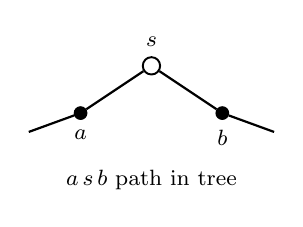
\begin{tikzpicture}[baseline]
      \node[cvertex,label={[glabel]below:$a$}] (a) at (-0.9,0) {};
      \node[cvertex,label={[glabel]below:$b$}] (b) at (0.9,0) {};
      \node[tvertex,label={[glabel]above:$s$}] (s) at (0,0.6) {};
      \draw[gedge] (a) -- (s) -- (b);
      \draw[gedge] (a) -- ++(200:0.7); \draw[gedge] (b) -- ++(340:0.7);
      \node[glabel] at (0,-0.85) {$a\,s\,b$ path in tree};
    \end{tikzpicture}}
  \end{subcaptionbox}
  \hfill
  \begin{subcaptionbox}{State (2): $e$ on a residual cycle, kept.\label{fig:state2}}[0.46\linewidth]{
    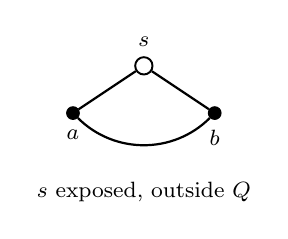
\begin{tikzpicture}[baseline]
      \node[cvertex,label={[glabel]below:$a$}] (a) at (-0.9,0) {};
      \node[cvertex,label={[glabel]below:$b$}] (b) at (0.9,0) {};
      \node[tvertex,label={[glabel]above:$s$}] (s) at (0,0.6) {};
      \draw[gedge] (a) -- (s) -- (b);
      \draw[gedge] (a) to[bend right=45] (b);
      \node[glabel] at (0,-1.0) {$s$ exposed, outside $Q$};
    \end{tikzpicture}}
  \end{subcaptionbox}

  \medskip

  \begin{subcaptionbox}{State (3): $e\in M_J$, endpoint in $Q$.\label{fig:state3}}[0.46\linewidth]{
    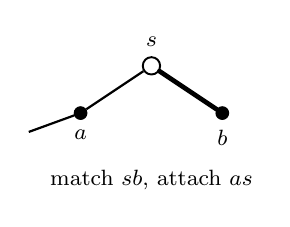
\begin{tikzpicture}[baseline]
      \node[cvertex,label={[glabel]below:$a$}] (a) at (-0.9,0) {};
      \node[cvertex,label={[glabel]below:$b$}] (b) at (0.9,0) {};
      \node[tvertex,label={[glabel]above:$s$}] (s) at (0,0.6) {};
      \draw[gedge] (a) -- (s);
      \draw[medge] (s) -- (b);
      \draw[gedge] (a) -- ++(200:0.7);
      \node[glabel] at (0,-0.85) {match $sb$, attach $as$};
    \end{tikzpicture}}
  \end{subcaptionbox}
  \hfill
  \begin{subcaptionbox}{State (4): $e\in M_J$, neither endpoint in $Q$.\label{fig:state4}}[0.46\linewidth]{
    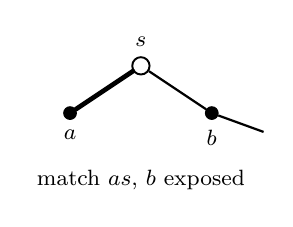
\begin{tikzpicture}[baseline]
      \node[cvertex,label={[glabel]below:$a$}] (a) at (-0.9,0) {};
      \node[cvertex,label={[glabel]below:$b$}] (b) at (0.9,0) {};
      \node[tvertex,label={[glabel]above:$s$}] (s) at (0,0.6) {};
      \draw[medge] (a) -- (s);
      \draw[gedge] (s) -- (b);
      \draw[gedge] (b) -- ++(340:0.7);
      \node[glabel] at (0,-0.85) {match $as$, $b$ exposed};
    \end{tikzpicture}}
  \end{subcaptionbox}
  \caption{The four states when restoring the suppressed path $a\,{-}\,s\,{-}\,b$.
  Heavy edges are matching edges. States (2) and (4) leave a single exposure $x$
  outside $Q$ and are resolved by \cref{lem:first-entry}.}
  \label{fig:restore-states}
\end{figure}


\section{Fragile graphs}\label{sec:fragile}

Suppose \cref{thm:simple-fragile} is false, and choose a counterexample $G$ with
the fewest vertices. A tree is
already a spanning-tree--matching decomposition, with empty matching, so $G$
contains a cycle.

First, $G$ has no bridge. If $b$ is a bridge and $G_1,G_2$ are the components of
$G-b$, then each $G_i$ is a smaller connected simple fragile subcubic graph. To
see fragility, a cycle whose edge deletion left $G_i$ connected would, after
restoring the other connected shore and the unchanged bridge, leave $G$
connected. By minimality, decompose each shore into a spanning tree $T_i$ and a
matching $M_i$. Then
\[
  T_1\cup\{b\}\cup T_2
\]
is a spanning tree of $G$, while $M_1\cup M_2$ is a matching because the shore
vertex sets are disjoint. Moreover $M_1\cup M_2$ is nonempty: if both $M_i$ were
empty, then both shores would be trees, and adjoining the bridge $b$ would make
$G$ itself a tree, contrary to the fact that $G$ contains a cycle. This is a
contradiction.

Thus $G$ is bridgeless. Since it is connected, cyclic and subcubic, all its
degrees are two or three. Put $k=\abs{\Vtwo(G)}$. Before applying
\cref{thm:terminal-selection}, we rule out $k=0$ and $k=1$.

If $k=0$, then $G$ is a simple cubic graph of even order $n\ge 4$. For any
$v\in V(G)$, let $c$ be the number of components of $G-v$. The sum of the
cyclomatic numbers of those components is
\[
  \left(\frac{3n}{2}-3\right)-(n-1)+c=\frac n2-2+c\ge 1 .
\]
Hence $G-v$ contains a cycle. Apply \cref{thm:protected-cycle} with $Q=\{v\}$.
Every vertex outside $Q$ has
ambient degree three, and the displayed cycle is in fact vertex-disjoint from
$Q$. The resulting removable cycle contradicts fragility.

If $k=1$, let $s$ be the unique terminal. Handshaking makes $n$ odd, and
simplicity forces $n\ge 5$. If $c$ is the number of components of $G-s$, the
total cyclomatic number is
\[
  \left(\frac{3n-1}{2}-2\right)-(n-1)+c=\frac{n-3}{2}+c\ge 1 .
\]
Thus $G-s$ contains a cycle. Protecting the connected one-vertex subgraph
$Q=\{s\}$ again satisfies the hypotheses of \cref{thm:protected-cycle}, because all vertices
outside $Q$ have ambient degree three. Fragility is again contradicted.

We therefore have $k\ge 2$. Apply \cref{thm:terminal-selection} to $G$. It
yields a matching $M$ such that $G-M$ consists of an all-terminal tree $Q$ and
some residual cycles. If a residual cycle exists, it is edge-disjoint (indeed
vertex-disjoint) from $Q$, and every vertex outside $Q$ has degree three in $G$,
because all degree-two vertices lie in $Q$. \Cref{thm:protected-cycle}
then supplies a cycle $C$ edge-disjoint from $Q$ for which $G-E(C)$ is
connected, contrary to fragility. Therefore there is no residual cycle: the tree
$Q$ is spanning, and $E(G)=E(Q)\dcup M$. This proves \cref{thm:simple-fragile}.

\section{The 2DC and 3DC conjectures}\label{sec:conjectures}

In this section graphs may have parallel edges but no loops, and a parallel pair
is a two-cycle.

\subsection{From the fragile theorem to 2DC}\label{sec:2dc-interface}

Let $\mathcal S_{2,3}$ be the class of finite connected loopless
multigraphs with every degree equal to two or three and every cycle separating.
The standard 2DC asks for a partition
\[
  E(G)=E(T)\dcup M,
\]
where $T$ is a spanning tree and $M$ is a nonempty matching.

For any $G\in\mathcal S_{2,3}$,
\[
  2\abs{E(G)}=2\abs{\Vtwo(G)}+3\abs{\Vthree(G)}=2\abs{V(G)}+\abs{\Vthree(G)},
\]
so every complementary spanning tree leaves
\begin{equation}\label{eq:matching-nonempty}
  \abs{E(G)}-\bigl(\abs{V(G)}-1\bigr)=\frac{\abs{\Vthree(G)}}{2}+1\ge 1
\end{equation}
edges in the matching part. The nonemptiness required by 2DC is therefore
automatic in this class.

Suppose 2DC were false, and choose a counterexample $G\in\mathcal S_{2,3}$
minimizing $\phi(G)=\abs{V(G)}+\abs{E(G)}$. By
\cref{thm:min-counterexample}, $G$ is simple and $2$-edge-connected,
hence a finite connected simple fragile subcubic graph.
\Cref{thm:simple-fragile} decomposes $G$ into a spanning tree and a
matching, a contradiction. This proves 2DC in its standard loopless-multigraph
form.

\subsection{From 2DC to 3DC}\label{sec:2dc-to-3dc}

The standard 3DC concerns finite connected cubic loopless multigraphs. A
$3$-decomposition is an edge partition
\[
  E(G)=E(T)\dcup E(C)\dcup M,
\]
where $T$ is a spanning tree, $C$ is a 2-regular subgraph, and $M$ is a
matching. The matching may be empty; the 2-regular part is necessarily nonempty
in a cubic graph, although this need not be imposed in the definition.

Let $G$ be a connected cubic loopless multigraph. Among all 2-regular subgraphs
$C$ for which
\[
  K:=G-E(C)
\]
is connected, choose one inclusion-maximal. The admissible family is nonempty
because the empty subgraph is admissible.

Let $H$ be the 2-core of $K$, obtained by repeatedly deleting vertices of
current degree at most one. If $H$ is empty, then $K$ is a connected forest and
hence a tree; $C$, that tree, and the empty matching already give a
$3$-decomposition.

Assume $H\ne\empt$. The 2-core is connected, since deleting a vertex of degree
at most one from a connected graph leaves the remaining nonempty graph
connected. Its degrees are two or three. Every vertex of $C$ has degree one in
$K$, because $G$ is cubic and $C$ uses exactly two of its incident edges; such a
vertex is deleted in the first pruning round, so
\begin{equation}\label{eq:VC-disjoint}
  V(C)\cap V(H)=\empt .
\end{equation}

The edges pruned from $K$ form a forest in which each tree component attaches to
$H$ exactly once. To see this, orient each deleted vertex's possible parent edge
toward its later-deleted neighbour. The deletion order precludes a directed
cycle, so the result is a forest terminating at $H$. If a component had two
attachment edges sharing a root in $H$, those two edges together with the forest
path between their outer endpoints would form a cycle, contradicting the deletion
of the outer vertex. Thus each pruned tree has exactly one attachment.

Every cycle of $H$ is separating in $H$. Otherwise, let $D$ be a cycle for which
$H-E(D)$ is connected. Restoring all rooted pruned trees shows that $K-E(D)$ is
connected. By \cref{eq:VC-disjoint}, $C\cup D$ is a strictly larger 2-regular
subgraph, and
\[
  G-E(C\cup D)=K-E(D)
\]
is connected, contrary to the maximal choice of $C$.

Thus $H\in\mathcal S_{2,3}$. Decompose $H$ into
a spanning tree $T_H$ and a matching $M$ by the result of
\cref{sec:2dc-interface}. Add every pruned forest edge to $T_H$. Because each
pruned tree has one attachment, the result is a spanning tree $T_K$ of $K$.
Consequently
\[
  E(G)=E(T_K)\dcup E(C)\dcup M
\]
is a $3$-decomposition of $G$, proving $\text{2DC}\Rightarrow\text{3DC}$. In any
such partition $C$ cannot be empty: otherwise the tree and matching would
contain at most $(\abs{V(G)}-1)+\abs{V(G)}/2<3\abs{V(G)}/2=\abs{E(G)}$ edges.

Together with \cref{sec:2dc-interface}, this proves 3DC for finite
connected cubic loopless multigraphs, establishing \cref{thm:3dc-resolved}.

\begin{remark}
  The converse implication also holds, giving the equivalence of
  Hoffmann-Ostenhof--Kaiser--Ozeki
  \cite[Proposition~14]{HoffmannOstenhofKaiserOzeki2018}. Given a 2DC instance
  $H$, attach to each degree-two vertex, by a bridge, a copy of the theta
  multigraph with one edge subdivided; the result is cubic and loopless. In any
  $3$-decomposition the attachment bridges lie in the tree, and each component
  of the $2$-regular part lies inside a theta copy, since a cycle through
  $E(H)$ stays separating while the $2$-regular part does not. Restricting the
  tree and matching to $H$ yields a $2$-decomposition, whose matching is
  nonempty by \cref{eq:matching-nonempty}.
\end{remark}


\section{Concluding remarks}\label{sec:scope}

\Cref{thm:terminal-selection} reduces 3DC to a question about matching
complements in simple subcubic graphs. We close with a question on the finer
structure of $3$-decompositions.

\begin{question}
  Fan, Guo, and Zhou~\cite{FanGuoZhou2026} showed that every connected cubic
  graph on $n$ vertices has a decomposition into a spanning tree, a 2-regular
  subgraph, and a collection of paths of length at most two, with at most
  $(n-4)/8$ paths of length two. Our result drives this count to zero. What is
  the extremal behaviour of other parameters of a $3$-decomposition---for
  instance, the minimum number of cycle components, or the maximum number of
  distinct $3$-decompositions as a function of $n$?
\end{question}


\section*{Acknowledgements}

The author thanks Luyi Li and Erling Wei for helpful discussions and
suggestions. The author used generative-AI tools during preliminary exploration
and language editing, and verified all mathematical statements and proofs, taking
full responsibility for the contents of the manuscript.

\begin{thebibliography}{99}

\bibitem{AbdolhosseiniAkbariHashemiMoradian2016}
F.~Abdolhosseini, S.~Akbari, H.~Hashemi, and M.~S. Moradian,
\emph{Hoffmann-Ostenhof's conjecture for traceable cubic graphs},
preprint (2016), \texttt{arXiv:1607.04768}.

\bibitem{AboomahigirAhanjidehAkbari2018}
E.~Aboomahigir, M.~Ahanjideh, and S.~Akbari,
\emph{Decomposing claw-free subcubic graphs and $4$-chordal subcubic graphs},
preprint (2018), \texttt{arXiv:1806.11009}.

\bibitem{BachtlerHeinrich2023}
O.~Bachtler and I.~Heinrich,
\emph{Reductions for the 3-Decomposition Conjecture},
Procedia Comput. Sci. \textbf{223} (2023), 96--103.

\bibitem{BachtlerKrumke2022}
O.~Bachtler and S.~O. Krumke,
\emph{Towards obtaining a 3-decomposition from a perfect matching},
Electron. J. Combin. \textbf{29} (2022), no.~4, Paper 4.23.

\bibitem{BorseWaphare2009}
Y.~M. Borse and B.~N. Waphare,
\emph{On removable cycles in connected graphs},
J. Indian Math. Soc. (N.S.) \textbf{76} (2009), no.~1--4, 31--46.

\bibitem{BorseWaphare2013}
Y.~M. Borse and B.~N. Waphare,
\emph{Removable cycles avoiding two connected subgraphs},
ISRN Discrete Math. \textbf{2013} (2013), Article ID 164535.

\bibitem{BotlerJimenezSambinelliWakabayashi2024}
F.~Botler, A.~Jim\'enez, M.~Sambinelli, and Y.~Wakabayashi,
\emph{On the structure of a smallest counterexample and a new class verifying
the 2-Decomposition Conjecture},
Graphs Combin. \textbf{40} (2024), Paper 102.

\bibitem{BoydIwataTakazawa2013}
S.~Boyd, S.~Iwata, and K.~Takazawa,
\emph{Finding 2-factors closer to TSP tours in cubic graphs},
SIAM J. Discrete Math. \textbf{27} (2013), no.~2, 918--939.

\bibitem{FanGuoZhou2026}
G.~Fan, S.~Guo, and C.~Zhou,
\emph{The 3-Decomposition Conjecture of cubic graphs},
Sci. China Math. \textbf{69} (2026), no.~8, 2239--2248.

\bibitem{FanZhou2025}
G.~Fan and C.~Zhou,
\emph{Hoffmann-Ostenhof's 3-decomposition conjecture},
Discrete Math. \textbf{348} (2025), no.~7, Article 114454.

\bibitem{HoffmannOstenhof2011}
A.~Hoffmann-Ostenhof,
\emph{Nowhere-zero flows and structures in cubic graphs},
Ph.D. thesis, University of Vienna, 2011.

\bibitem{HoffmannOstenhofKaiserOzeki2018}
A.~Hoffmann-Ostenhof, T.~Kaiser, and K.~Ozeki,
\emph{Decomposing planar cubic graphs},
J. Graph Theory \textbf{88} (2018), no.~4, 631--640.

\bibitem{HongLiuYu2020}
Y.~Hong, Q.~Liu, and N.~Yu,
\emph{Edge decomposition of connected claw-free cubic graphs},
Discrete Appl. Math. \textbf{284} (2020), 246--250.

\bibitem{LiCui2014}
R.~Li and Q.~Cui,
\emph{Spanning trees in subcubic graphs},
Ars Combin. \textbf{117} (2014), 411--415.

\bibitem{LiuLi2020}
P.~Li and W.~Liu,
\emph{Decompositions of cubic traceable graphs},
Discuss. Math. Graph Theory \textbf{40} (2020), no.~1, 35--49.

\bibitem{LyngsieMerker2019}
K.~S. Lyngsie and M.~Merker,
\emph{Decomposing graphs into a spanning tree, an even graph, and a star
forest},
Electron. J. Combin. \textbf{26} (2019), no.~1, Paper 1.33.

\bibitem{Malkevitch1979}
J.~Malkevitch,
\emph{Spanning trees in polytopal graphs},
Ann. New York Acad. Sci. \textbf{319} (1979), 362--367.

\bibitem{OzekiYe2016}
K.~Ozeki and D.~Ye,
\emph{Decomposing plane cubic graphs},
European J. Combin. \textbf{52} (2016), 40--46.

\bibitem{Petersen1891}
J.~Petersen,
\emph{Die Theorie der regul\"aren Graphs},
Acta Math. \textbf{15} (1891), 193--220.

\bibitem{ProttiSouza2018}
F.~Protti and U.~S. Souza,
\emph{Decycling a graph by the removal of a matching: new algorithmic and
structural aspects in some classes of graphs},
Discrete Math. Theor. Comput. Sci. \textbf{20} (2018), no.~2, Paper 15.

\bibitem{Schonberger1935}
T.~Sch\"onberger,
\emph{Ein Beweis des Petersenschen Graphensatzes},
Acta Sci. Math. (Szeged) \textbf{7} (1935), 51--57.

\bibitem{XieZhouZhou2020}
M.~Xie, C.~Zhou, and S.~Zhou,
\emph{Decomposition of cubic graphs with a 2-factor consisting of three cycles},
Discrete Math. \textbf{343} (2020), 111839.

\bibitem{ZhangSzeider2025}
T.~Zhang and S.~Szeider,
\emph{The 3-Decomposition Conjecture: a SAT-based approach with specialized
propagators},
in \emph{31st International Conference on Principles and Practice of Constraint
Programming (CP 2025)}, LIPIcs \textbf{340}, 2025, pp. 39:1--39:19.

\end{thebibliography}

\end{document}
